\subsubsection{Ballnachschub}
\begin{figure}[h!]
	\centering
	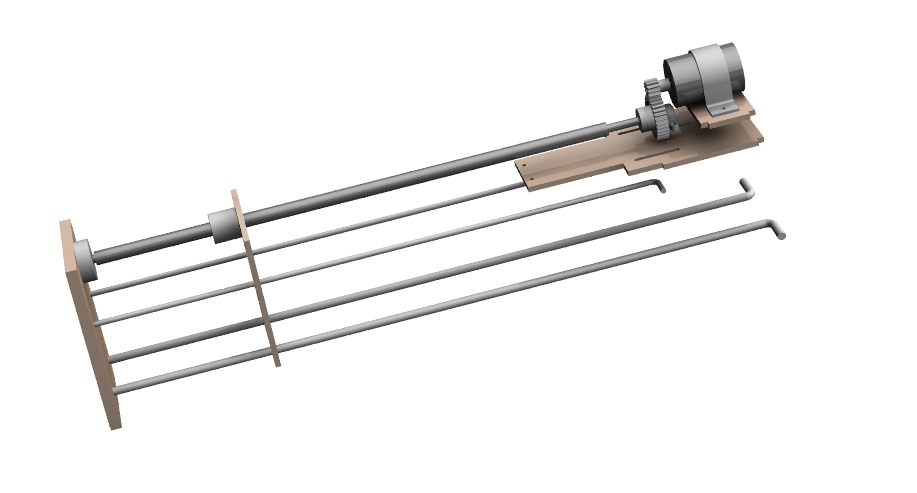
\includegraphics[width=\linewidth]{../../fig/Ballnachschub}
	\caption{Ballnachschub}
	\label{fig:Ballnachschub}
\end{figure}
\paragraph{Komponentenbeschrieb\\}
Der Ballnachschub wird mit einer rotierenden Trapezgewindespindel (TR10x3) und einem Mitnehmer sichergestellt. Die Tennisbälle werden seitlich mit Alustangen geführt und so in Richtung der Abwurfvorrichtung transportiert. Die Trapezgewindespindel ist auf der Unterseite mit einem Rillenkugellager gelagert. Auf der Oberseite wird die Lagerung mit einem Stehlager aus Kunststoff der Firma Igus realisiert. Ein DC-Motor treibt die Trapezgewindespindel an. Die Kraftübertragung vom DC-Motor auf die Trapezgewindespindel erfolgt mit zwei Kunststoff Stirnrädern. Das Übersetzungsverhältnis hierbei beträgt 2.67.

\paragraph{Entwicklungsprozess\\}
In einem ersten Entwurf wurde die Trapezgewindeführung auf der Unterseite auch mit einer Gleitführung realisiert. Dies funktionierte für den Ballnachschub einwandfrei. Wurde nach dem Ballabwurf die Drehrichtung umgekehrt, um den Mitnehmer zurück in die Startposition zu bringen, ergaben sich jedoch einige Probleme. Wegen der realisierten Gleitführung konnte sich die Trapezgewindespindel in axialer Richtung frei bewegen. Dies führte dazu, dass die Spindel beim Zurückstellen tendenziell nach oben gezogen wurde. Dies führte zu hörbaren Schwingungen, welche ein automatisches Zurückfahren erschwerten. Mit der angepassten Lagerung tritt dieses Problem nicht mehr auf. 
Eine weitere Knacknuss war die Führung der Bälle und dadurch das Finden der optimalen Position für die Führungsstangen. Da Tennisbälle eine runde Form besitzen, neigen sie dazu sich gegenseitig wegzudrücken. Daher mussten wir vier Aluminiumstangen als Führung verwende. In einer ersten Version waren nur zwei Stangen auf der Unterseite vorgesehen. Beim ersten Entwurf endeten alle Führungsstangen auf der Höhe des Drehrades. Dies führte dazu dass die Tennisbälle nach dem Abwurf, die Maschine auf einer horizontalen Flugbahn verliessen und nicht wie vorgesehen unter einem Winkel von 45° zur Horizontalen. Dieses Problem konnte durch einer Verlängerung der Führungsstangen bis nach dem Drehrad verhindert werden. 
Der DC Motor wird mit einer Rohrschelle befestigt. Dabei wurde die Platte, auf welcher die Rohrschelle befestigt ist, im richtigen Abstand positioniert, so dass die Übersetzung realisiert werden kann. Dies stellt keine optimale Lösung dar. Da die Funktion jedoch erfüllt ist, wird auf eine Verbesserung verzichtet. 
